\documentclass[tikz,border=10pt]{standalone}
\usepackage{amsmath}
\usepackage{amssymb}
\usetikzlibrary{calc, arrows.meta}

\definecolor{vecgreen}{HTML}{2E7D32}  
\definecolor{vecblue}{HTML}{1565C0}   
\definecolor{vecdark}{HTML}{212121}   
\definecolor{surfbg}{HTML}{9E9E9E}

\begin{document}
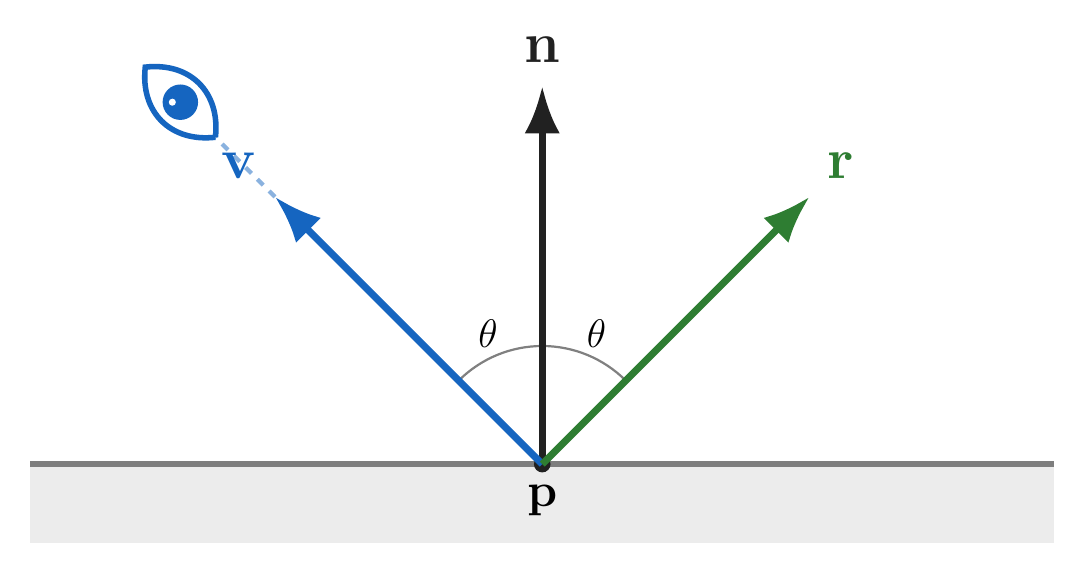
\begin{tikzpicture}[
    vec/.style={line width=2.5pt},
    >={Latex[length=6mm, width=4.5mm]}
]

\pgfmathsetmacro{\Vangle}{135}   
\pgfmathsetmacro{\Rangle}{45}    
\pgfmathsetmacro{\vecLen}{4.8}
\pgfmathsetmacro{\EyeDist}{6.5}

% Surface
\fill[surfbg!20] (-6.5, -1) rectangle (6.5, 0);
\draw[line width=2pt, surfbg!80!black] (-6.5, 0) -- (6.5, 0);

% Origin
\coordinate (O) at (0,0);
\fill[vecdark] (O) circle (3pt);
\node[below=4pt, font=\LARGE] at (O) {$\mathbf{p}$};

% Angles
\draw[gray, thick] (90:1.5) arc (90:\Vangle:1.5);
\node[font=\Large] at (112.5:1.8) {$\theta$};
\draw[gray, thick] (90:1.5) arc (90:\Rangle:1.5);
\node[font=\Large] at (67.5:1.8) {$\theta$};

% Normal
\draw[->, vec, vecdark] (O) -- (90:\vecLen) node[above=4pt, font=\huge] {$\mathbf{n}$};

% View Ray
\coordinate (Vtip) at (\Vangle:\vecLen);
\draw[->, vec, vecblue] (O) -- (Vtip) node[above left=2pt, font=\huge] {$\mathbf{v}$};

% Reflection Ray
\coordinate (Rtip) at (\Rangle:\vecLen);
\draw[->, vec, vecgreen] (O) -- (Rtip) node[above right=2pt, font=\huge] {$\mathbf{r}$};

% Viewer (Eye) Context
\coordinate (EyePos) at (\Vangle:\EyeDist);
\draw[line width=1.5pt, vecblue, dashed, opacity=0.5] (Vtip) -- (EyePos);
\begin{scope}[shift={(EyePos)}, rotate=\Vangle, scale=0.9]
    \fill[white] (0,0) ellipse (0.7 and 0.4);
    \draw[line width=2pt, vecblue] (-0.7,0) .. controls (-0.3,0.5) and (0.3,0.5) .. (0.7,0)
                            .. controls (0.3,-0.5) and (-0.3,-0.5) .. (-0.7,0);
    \fill[vecblue] (0,0) circle (0.25);
    \fill[white] (0.08,0.08) circle (0.05); 
\end{scope}

\end{tikzpicture}
\end{document}